\documentclass[11pt,a4paper,english,oneside]{book}
\usepackage{url}
\usepackage{latexsym}

\usepackage[onehalfspacing]{setspace}
\usepackage[top=1in,bottom=1in,left=1.5in,right=1in]{geometry}

\usepackage{fontspec}
\defaultfontfeatures{Ligatures=TeX}
\usepackage{sectsty}
\allsectionsfont{\normalfont}
\paragraphfont{\bfseries}
\setmainfont[
BoldFont=texgyrepagella-bold.otf,
ItalicFont=texgyrepagella-italic.otf,
BoldItalicFont=texgyrepagella-bolditalic.otf]
{texgyrepagella-regular.otf}

\usepackage[round,sort]{natbib}

\usepackage{subcaption}
\usepackage{booktabs}
\usepackage{amsmath}
\usepackage{multirow}
\usepackage{paralist}
\usepackage[parfill]{parskip}
\usepackage{todonotes}
\usepackage{wrapfig}

\usepackage{csquotes}
\renewcommand{\mkcitation}[1]{ #1}

\usepackage{tikz}
\usepackage{tikz-qtree}

\usepackage{listings}
\usepackage{color}
\usepackage{textcomp}
\definecolor{listinggray}{gray}{0.9}
\definecolor{lbcolor}{rgb}{0.9,0.9,0.9}
\lstset{
  captionpos=b,
  basicstyle=\ttfamily,
  keywordstyle=\color[RGB]{66, 54, 122},
}

% \clubpenalty=10000
% \widowpenalty = 10000

\usepackage{hyperref}
\def\UrlBreaks{\do\/\do-}

% \title{Categorical Composition Models in Large Scale NLP Tasks}
% \title{Bringing Semantics to NLP Tasks Using Categorical Composition}
% \title{Scaling Up Distributional Semantics to Real World NLP Tasks Using Categorical Composition}
% \title{The Role of Computers in Understanding Natural Language}
\title{What Computers Should Know about Texts}
\author{Dmitrijs Milajevs}
% \affil{Queen Mary University of London}

% http://colorschemedesigner.com/#4o42FfqublRMS
\definecolor{linkcolor}{RGB}{66, 54, 122}
\definecolor{citecolor}{RGB}{84, 141, 100}
\definecolor{urlcolor}{RGB}{168, 70, 67}
\hypersetup{
  colorlinks=true,
  linkcolor=linkcolor,
  citecolor=citecolor,
  urlcolor=urlcolor,
  pdftitle=\@title,
  pdfauthor={Dmitrijs Milajevs},
}

\DeclareMathOperator{\my-c}{count}
\newcommand{\ov}{\overrightarrow}

\newcommand\newcite\citet
\renewcommand\cite\citep

\begin{document}
% \maketitle
% \addtocounter{page}{1}

% \chapter*{Statement of originality}

I, Dmitrijs Milajevs, confirm that the research included within this thesis is my own work or that where it has been carried out in collaboration with, or supported by others, that this is duly acknowledged below and my contribution indicated. Previously published material is also acknowledged below.

I attest that I have exercised reasonable care to ensure that the work is original, and does not to the best of my knowledge break any UK law, infringe any third party’s copyright or other Intellectual Property Right, or contain any confidential material.

I accept that the College has the right to use plagiarism detection software to check the electronic version of the thesis.

I confirm that this thesis has not been previously submitted for the award of a degree by this or any other university.

The copyright of this thesis rests with the author and no quotation from it or information derived from it may be published without the prior written consent of the author.

Signature:

Date: \today

Details of collaboration and publications:
\begin{enumerate}
\item \citet*{milajevs-purver:2014:CVSC}
\item \citet*{milajevs-EtAl:2014:EMNLP2014}
\item \citet*{Milajevs:2015:IMN:2808194.2809448}
\item \citet*{milajevs:2016:SRW1}
\item \citet*{milajevs-griffiths:2016:repeval}
\end{enumerate}

%%% Local Variables:
%%% mode: latex
%%% TeX-master: "thesis"
%%% End:
\cleardoublepage

% {\Large \headingfont \thetitle}

\vspace{1em}

{\large \headingfont \theauthor}

\vspace{1em}

{\headingfont Abstract}

Representation of sentences that captures semantics is an essential part of natural language processing systems, such as information retrieval or machine translation. The representation of a sentence is commonly built by combining the representations of the words that the sentence consists of. Similarity between words is widely used as a proxy to evaluate semantic representations. Word similarity models are well-studied and are shown to correlate with human judgements.
% * <sdyck@ualberta.ca> 2017-03-01T01:58:25.286Z:
% 
% > correlate
% In what way? positively?
% 
% ^.

Current evaluation of models of sentential similarity builds on the results obtained in lexical experiments. The main focus is how the lexical representations are used, rather than what they should be. It is often assumed that the optimal representations for word similarity are also optimal for sentence similarity. This work discards this assumption and systematically looks for lexical representations that are optimal for similarity measurement between sentences.

We find that the best representation for word similarity is not always the best for sentence similarity and vice versa. The best models in word similarity tasks perform best with additive composition. However, the best result on compositional tasks is achieved with Kronecker-based composition. There are representations that are equally good in both tasks when used with multiplicative composition.

The systematic study of the parameters of similarity models reveals that the more information lexical representations contain, the more attention should be paid to noise. In particular, the word vectors in models with the feature size at the magnitude of the vocabulary size should be sparse, but if a small number of context features is used then the vectors should be dense.

Given the right lexical representations, compositional operators achieve state-of-the-art performance, improving over models that use neural-word embeddings. To avoid overfitting, either several test datasets should be used or parameter selection should be based on parameters' average behaviours.

\vfill

%Submitted in partial fulfillment of the requirements of the Degree of Doctor of Philosophy

Submitted for the degree of Doctor of Philosophy

Queen Mary University of London

\today


%%% Local Variables:
%%% mode: latex
%%% TeX-master: "thesis"
%%% End:
\cleardoublepage

\tableofcontents\cleardoublepage

\todototoc
\listoftodos

\chapter{Introduction}
\label{ch:introduction}

Computers require specially designed programming languages to be controlled, despite the fact that they play a crucial role in our lives. Ideally, the interaction with a computer should not be different from the interaction with a human. Computational linguistics is one of the fields that addresses this problem.

Computers need to understand human language in order to be controlled by people in a casual manner. However, different tasks require various levels of language understanding. For instance, even if one does not recognise or know the language of a piece of text in Figure~\ref{fig:lv}, one can tell that there are 39 words and that there is only one sentence. One can even argue that this is a piece of poetry and the first line is its title basing the argument on the shape of the text.

The conclusions above require neither the complete understanding of the language nor the meaning of the text. The knowledge that texts---at least in some languages---consist of words separated by a space and how poems are written is enough. Moreover, knowing the letter distribution across all human languages or having a list of words in them, one would conclude that the text is in Latvian. This information can be provided without knowing what the text is about and are currently successfully done by computers.

\begin{figure}[t]
\tiny
\begin{subfigure}[t]{0.30\textwidth}
  Jaunkundze ar sunīti \\

  Un Vecrīgas šķērsielā, šaurā \\
  kā vēstuļu kastītes sprauga, \\
  kur troksnim un burzmai tik atbalss, \\
  kur smaržo pēc darvas, \\ ${}$\qquad dzelzs un pēc āboliem pagrabos sausos, \\
  es satiku jaunkundzi -- \\
  glītu un veiklu kā mēle, \\
  kā spēlējot vijoles lociņš.
  \vspace{0.74cm}
  \caption{}
  \label{fig:lv}
\end{subfigure}
~
\begin{subfigure}[t]{0.36\textwidth}
  Барышня с собачкой \\

  В Старой Риге, на улице поперечной, узкой, \\
  как щель в почтовый ящик, \\
  в который проникают только отголоски шума, гама, \\
  где запах дёгтя, ржавчины и яблок в сухих  подвалах, \\
  я встретил барышню -- \\
  красива и ловка - она - язык, \\
  смычок, играющий на скрипке.
  \vspace{0.99cm}
  \caption{}
  \label{fig:ru}
\end{subfigure}
~
\begin{subfigure}[t]{0.26\textwidth}
  Young Woman with a Dog \\

  On a narrow side-street in Riga’s old quarter, \\
  as though in a mailbox slot \\
  where noise and hustle only echo, \\
  and it smells of tar and steel \\
  and apples kept in dry basements, \\

  I met a young woman \\
  attractive and active \\
  as a tongue, \\
  as a violin-bow playing.
  \caption{}
  \label{fig:en}
\end{subfigure}
\caption[Three pieces of written natural language.]{Three pieces of written natural language. The text on
  Figure~\ref{fig:lv} is the beginning of the poem ``Jaunkundze ar sunīti'' by
  Aleksandrs Čaks, Figure~\ref{fig:ru} is a translation to Russian by Lora Trin,
  and Figure~\ref{fig:en} is an English translation by Inara Cedrins.}
\end{figure}


On the other hand, a task that asks for a list of associations, an essay or a painting inspired by a piece of text demands a much better understanding of the text that requires a deeper knowledge of the language and greater familiarity with the culture. Luckily, nowadays these kinds of tasks are not expected to be completed by computers in day-to-day life because people enjoy doing these things themselves.

However, it is reasonable to ask a computer the following questions regarding the text:
\begin{inparaenum}[a)]
\item What is the text of Figure~\ref{fig:lv} about?
\item What is the relationship between the texts in Figure~\ref{fig:lv} and
  Figure~\ref{fig:ru}?
% the *meanings are identical*
\item Is the content similar or identical?
\item Where did the meeting take place?
\item What poems are similar to this?
\end{inparaenum}

Text summarisation, machine translation, information extraction and information retrieval are branches of computational linguistics that provide methods for answering these questions. The questions above have a general property: all of them are about a certain aspect of the meaning of the text. Semantics is an area that studies meaning representation and thus, is necessary to solve these tasks.

While it is not completely known how meaning is represented in the human mind, it is argued that similarity between two events or objects is based on the way humans represent them \cite{WCS:WCS1282}. Similarity judgements are easy to collect. Many similarity datasets exist that serve as proxies for evaluation of computational models of meaning.

The distributional hypothesis of \citet{harris1954distributional}---that semantically similar words tend to appear in similar contexts---stands behind the distributional models of meaning. In Figure~\ref{fig:en}, the side-street occurs with the words as \textit{slot}, \textit{noise}, \textit{hustle} and \textit{smells}. Such a company of words starkly contrasts with the words used to describe the woman: she is young, attractive and active.

Moreover, the descriptive neighbouring words of the side-street bring images of other things similar to it that are noisy and smell. At the same time, the descriptive terms of the woman fire in the mind attractive and active associations making the difference between the street and the woman even stronger!

Distributional models of word meaning (also known as lexical models of meaning) are based on the co-occurrence statistics of words in a large collection of texts \cite{Turney:2010:FMV:1861751.1861756,mikolov2013linguistic,mikolov2013distributed,mikolov2013efficient}. The main challenge is to use the co-occurrence statistics efficiently. Because, even though the word \textit{and} appears in the neighbourhood of the word \textit{side-street} in the poem, it is much less descriptive of the properties of the street than the word \textit{slot}. Nowadays, the lexical models are well studied and their estimates of the similarity between word pairs are very close to the human judgements \cite{TACL570,baroni-dinu-kruszewski:2014:P14-1,Halawi:2012:LLW:2339530.2339751}.

The estimation of the similarity of multi-word expressions currently is an active research topic. In comparison to the lexical models, the main challenge is the data sparsity. There are infinitely many multi-word expressions and most of them appear only once in a corpus. Even if we take all the books on Earth and write down all the utterances that were said, the most of the sentences appear only once.

The dominant solution to the data sparsity problem is to build a representation of a multi-word expression compositionally: that is, the same way the Lego pieces are assembled into vehicles, buildings and many other types of objects. One advantage of such an approach is that the methods for obtaining the word representations can be reused. The bricks are there, the question is how to assemble them together.

The compositional models come in many flavors. \citet{mitchell2010composition} propose a method that ignores the word order and any grammatical structure of an expression. \citet{DBLP:journals/corr/abs-1003-4394,baroni2014frege} investigate how the grammatical structure can be taken into account. Several implementations of \citet{DBLP:journals/corr/abs-1003-4394}'s theoretical proposal exist, see the work of \citet{Grefenstette:2011:ESC:2145432.2145580,Grefenstette:2011:ETV:2140490.2140497,kartsadrqpl2014,fried-polajnar-clark:2015:ACL-IJCNLP}. Chapter~\ref{cha:background} gives an overview of lexical representations, the methods of composition and evaluation.

The main focus of the evaluation of compositional similarity models up to now is the compositional operators. The word representations are usually taken such that they are good in lexical tasks. The fact that there might be a dependency between the word representations and the compositional methods is mostly overlooked. It is assumed, that the findings based on the lexical models also applies to the compositional models.

The goal of this thesis is to study the link between the lexical representations and the methods of composition for similarity estimation. Once the optimal lexical parameters are identified for all compositional operators, the operators can be compared in the most fair way.

The goal is expressed in two research questions:
\begin{itemize}
\item What is the performance limit of the distributional models of meaning?
\item How are compositional operators affected by the lexical representations?
\end{itemize}

To answer these questions, we perform a large-scale study of similarity models over several parameters. The parameters are split into three kinds: the similarity measure, the weighting scheme and the amount of information associated with every item. 

The similarity measure defines how similarity is computed given two representations. The weighting scheme serves two roles. First of all, it distinguishes informative co-occurrence information from uninformative. Second, the weighting scheme minimises the effect of noise in the co-occurrence data. The amount of information for distributional modes is how many distinct words are considered to be valid neighbouring words. This usually varies from few thousand most frequent words to the whole vocabulary.  The description of model parameters is given in Chapter~\ref{sec:methodology}.

We extensively test composition based on point-wise addition and multiplication of the weighted co-occurrence counts to identify the best lexical representations for composition (Chapters~\ref{sec:sentential} and \ref{sec:universal-param-selection}). We find that indeed, there is a link between the compositional operators and lexical representations.

By taking into account the dependency between the compositional operator and the lexical representation,  we achieve the state of the art results with additive and multiplicative composition. By reusing the best lexical representations with categorical compositional operators \cite{DBLP:journals/corr/abs-1003-4394}, we improve their performance. Moreover, we show that the optimal parameters to measure the similarity between words (Chapter~\ref{sec:lexical}) are different from the optimal parameters to measure similarity between phrases.

\section{Structure of this thesis}
\label{sec:structure}

\textbf{Chapter~\ref{cha:background}} A review of logical and distributional models of meaning. Description of the current similarity datasets and an overview of the current state of the art models.

\textbf{Chapter~\ref{sec:methodology}} The methodology for robust selection of similarity models. The description of used model parameters. The list of hypotheses.

\textbf{Chapter~\ref{sec:lexical}} Experiments of the lexical datasets: SimLex-999 and MEN.

\textbf{Chapter~\ref{sec:phraserel}} Description of PhraseRel, a new phrase relevance dataset.

\textbf{Chapter~\ref{sec:sentential}} Experiments on three phrasal datasets: GS11, KS14 and PhraseRel.

\textbf{Chapter~\ref{sec:universal-param-selection}} selection of the models based on all datasets. Experiments with tensor-based compositional methods.

\textbf{Chapter~\ref{cha:conclusion}} Conclusion of the thesis.

%%% Local Variables:
%%% mode: latex
%%% TeX-master: "thesis"
%%% TeX-engine: xetex
%%% End:

\chapter{Overview}
% \label{cha:similarity}

\section{Similarity}
\label{sec:similarity}

Similarity is the degree of resemblance between two objects or events \cite{WCS:WCS1282} and plays a crucial role in psychological theories of knowledge and behaviour, where it is used to explain such phenomena as classification and conceptualisation \cite{Tversky1977,1986-13502-00119860101,medin1993respects,Markman1996,hahn1997concepts}. \textit{Fruit} is a \emph{category} because it is a practical generalisation. Fruits are sweet and constitute deserts, so when one is presented with an unseen fruit, one can hypothesise that it is served toward the end of a dinner.

Generalisations are extremely powerful in describing a language as well. The verb \textit{runs} requires its subject to be singular. \textit{Verb}, \textit{subject} and \textit{singular} are categories that are used to describe English grammar. When one encounters an unknown word and is told that it is a verb, one will immediately have an idea about how to use it assuming that it is used similarly to other English verbs.

From a computational perspective, this motivates and guides development of similarity components that are embedded into natural language processing systems that deal with tasks such as
word sense disambiguation \cite{Schutze:1998:AWS:972719.972724},
information retrieval \cite{Salton:1975:VSM:361219.361220,Milajevs:2015:IMN:2808194.2809448},
machine translation \cite{Dagan:1993:CWS:981574.981596},
dependency parsing \cite{hermann-blunsom:2013:ACL2013,andreas-klein:2014:P14-2},
dialogue act tagging \cite{kalchbrenner-blunsom:2013:CVSC,milajevs-purver:2014:CVSC},
reasoning over knowledge bases \cite{NIPS2013_5028},
and language modelling \cite{bengio2006}.

Concretely, a parser might benefit from a generalisation about the part of speech tag of a word which did not occur in the training data based on its occurrence pattern in a large corpus of documents from the web. A dialogue act tagging system, contrastly, might require to classify a whole sentence based on its role in a dialogue. To be useful, the similarity component has to be able to measure similarity between \emph{words} and \emph{sentences}.

According to \newcite{WCS:WCS1282} ``similarity is an essentially psychological notion, based on the way we represent objects, that is, the way they appear to us.'' An important consequence of this observation is that before measuring similarity of two
\todo{What's the general term for events and objects? Entity?}%
entities,\footnotemark{} their representation has to be obtained.

\footnotetext{Here and later \emph{entity} is a common term for \textit{events} and \textit{objects}.}

% \cite{Huth2016}

\section{Entity representation for similarity measurement}
\label{sec:word-meaning}

Section \ref{sec:similarity} established that before measuring similarity, the representation of entities has to be agreed. One needs to be extremely careful when the representation of lexical items is decided, as it is unavoidably connected to the \emph{meaning words in isolation}.

% The semantic formalisation of similarity is based on two ideas. The occurrence pattern of a word \emph{defines} its meaning \cite{firth1957lingtheory}, while the difference in occurrence between two words \emph{quantifies} the difference in their meaning \cite{harris1954distributional}.

Frege discusses two conflicting principles of meaning \cite{Janssen2001}. Isolated words meanings are the building blocks of sentence meanings, according to \emph{the principle of compositionality}:
\begin{displayquote}[\cite{Janssen2001}]
The meaning of a compound expression is a function of the meaning of its parts and the syntactic rule by which they are combined.
\end{displayquote}
But the word meaning in isolation is not defined, according to \emph{the principle of contextuality}:
\begin{displayquote}[\cite{Janssen2001}]
Never ask for the meaning of a word in isolation, but only in the context of a sentence.
\end{displayquote}

It worth noting here, that similarity in isolation is also problematic because the number of features an entity has is infinite and its easy to show that two entities will always have an infinite amount of common features \cite{goodman1972problems,hahn1997concepts}. To make similarity measurement possible, it has to be measured \emph{under a given description} \cite{WCS:WCS1282,medin1993respects,Markman1996}, thus similarity is always contextualised. Also, \newcite{Huth2016} were able to comprehensively map individual words across cortex, meaning that there are word representations.

Frege's principle of contextuality allows to define the meaning of a word by identifying its contribution to the meaning of a sentence. Firth's \citeyearpar{firth1957lingtheory} famous quote that ``you shall know a word by the company it keeps''  suggests that the word meaning can be \emph{modelled} as the combination of the meanings of its occurrences in sentences of a corpus. Note, that this does not provide the absolute word meaning, but only its meaning relative to the corpus. This assumption is also supported by the hypothesis of \newcite{harris1954distributional} that the differences of occurrences of two words \emph{quantify} the difference in their relative meanings.

Once relative word meaning is accepted, compositionality can be used to obtain representations of phrases and sentences \cite{THEO:THEO373,Dowty1980,sep-montague-semantics,DBLP:journals/corr/abs-1003-4394,baroni2014frege}.

\section{Distributional hypothesis}
\label{sec:distr-hypoth}

We would like to capture the intuition that while \textit{John} and \textit{Mary} are distinct, they are rather similar to each other (both of them are humans) and dissimilar to \textit{dog}, \textit{pavement} or \textit{idea}.

% The same applies at the phrase and sentence level: \textit{dogs chase cats} is similar in meaning to \textit{hounds pursue kittens}, but less so to \textit{cats chase dogs} (despite the lexical overlap).

Distributional methods provide a way to approach this problem. By representing words and phrases as vectors in a vector space, we can express similarity in meaning via a suitable distance metric within that space.

\subsection{Co-occurrence based word representation}
\label{sec:distr-repr}

One way to produce such representations is to directly exploit Harris' \citeyearpar{harris1954distributional} intuition by counting the contexts a word appears in.

% that semantically similar words tend to appear in similar contexts.

For example, one can construct a vector space in which the dimensions correspond to contexts, that are usually other words. The word vector components can then be calculated by taking the frequency with which the word co-occurred with the corresponding contexts within a predefined window in a corpus of interest.

\begin{wraptable}[10]{O}{7cm}
  \centering
  \begin{tabular}{lrrr}
    \toprule
    & philosophy & book & school \\
    \midrule
    John & 4  & 60 & 59  \\
    Mary & 0  & 10 & 22  \\
    girl & 0  & 19 & 93  \\
    boy  & 0  & 12 & 146 \\
    idea & 10 & 47 & 39  \\
    \bottomrule
  \end{tabular}
  \caption{Word co-occurrence frequencies extracted from the BNC.}
  \label{tab:comparison}
\end{wraptable}

Table~\ref{tab:comparison} shows 5 3-dimensional vectors for the words \textit{Mary}, \textit{John}, \textit{girl}, \textit{boy} and \textit{idea}. The words \textit{philosophy}, \textit{book} and \textit{school} label vector space dimensions.

As the vector for \textit{Mary} is \todo{Is it accurate to talk about vector closeness?}closer to \textit{girl} than it is to \textit{boy} in the vector space, we can say that \textit{Mary}'s contexts are similar to \textit{girls}'s (and less similar to \textit{boy}'s), therefore \textit{Mary} is semantically more similar to \textit{girl} than to \textit{boy}.

Mathematically the similarity can be expressed using, for instance, the cosine of the angle between two vectors:
%
\begin{align*}
\cos(\theta) &=
\frac{\ov{\mathit{Mary}}\cdot\ov{\mathit{girl}}}
{||\ov{\mathit{Mary}}||\ov{\mathit{girl}}||} =
%
\frac{0\times0 + 10\times19 + 22\times93}
{\sqrt{0^2 + 10^2 + 22^2}\sqrt{0^2 + 19^2 + 93^2}} \approx
\frac{2236}{2294} \approx 0.975
 \\
\cos(\phi) &=
\frac{\ov{\mathit{Mary}}\cdot\ov{\mathit{boy}}}
{||\ov{\mathit{Mary}}||\ov{\mathit{boy}}||} =
%
\frac{0\times0 + 10\times12 + 22\times146}
{\sqrt{0^2 + 10^2 + 22^2}\sqrt{0^2 + 12^2 + 146^2}} \approx
\frac{3332}{3540} \approx 0.941
\end{align*}
%
where $\theta$ is the angle between the vectors of \textit{Mary} and \textit{girl}; and $\phi$ is the angle between the vectors of \textit{Mary} and \textit{boy}.

In the current example of a na{\"i}ve example vector space, \textit{John} is also closer to \textit{girl} than to \textit{boy}, which is counter-intuitive. This might be because of the small number of dimensions used, the poor selection of the context words, or the usage of raw co-occurrence numbers. Refer to \newcite{Turney:2010:FMV:1861751.1861756} and \newcite{TACL570} for the discussion of vector space parameters, and see \newcite{kiela-clark:2014:CVSC}, \newcite{lapesa2014large} and
%
\todo{reference the section about parameters} below
%
for a detailed comparison of their tuning and performance.

\subsection{Neural word embedding}
\label{sec:neural-embedding}

Deep learning techniques use this distributional hypothesis
differently. Instead of relying on observed co-occurrence frequencies,
a neural model is trained to maximise some objective function related
to e.g. the probability of observing the surrounding words in some
context \cite{mikolov2013distributed}:
%
\begin{align}
 \frac{1}{T}\sum^{T}_{t=1}\sum_{-c \leq j \leq c, j\neq0} \log p(w_{t+j}|w_t)
  \label{eq:objective-func}
\end{align}
%
\noindent
Maximising this function produces vectors which maximise the
conditional probability of observing words in a context around the
target word $w_t$, where $c$ is the size of the training context, and
$w_1 w_2, \cdots w_T$ is a sequence of training words. They therefore
capture the distributional intuition and can express degrees of
lexical similarity.

% Explain why is this better than counting

They have also proved successful at other tasks \cite{mikolov2013linguistic}; the vectors obtained encode not only attributional similarity (similar words are close to each other), but also relational similarities \cite{Turney:2010:FMV:1861751.1861756}. For example, it is possible to extract the \texttt{singular:plural} relation (\textit{apple}:\textit{apples}, \textit{car}:\textit{cars}) using vector subtraction:
%
\begin{align*}
  \overrightarrow{\mathit{apple}} - \overrightarrow{\mathit{apples}}
  \approx
  \overrightarrow{\mathit{car}} - \overrightarrow{\mathit{cars}}
\end{align*}
%
also semantic relationships are preserved:
%
\begin{align*}
  \overrightarrow{\mathit{king}} - \overrightarrow{\mathit{man}}
  \approx
  \overrightarrow{\mathit{queen}} - \overrightarrow{\mathit{woman}}
\end{align*}
%
allowing the formation of analogy queries similar to
$\overrightarrow{\mathit{king}} - \overrightarrow{\mathit{man}} +
\overrightarrow{\mathit{woman}} = \mathtt{?}$, obtaining
$\overrightarrow{\mathit{queen}}$ as the
result.\footnote{\newcite{levy2014linguistic} improved
  \newcite{mikolov2013linguistic}'s method of retrieving relational similarities
  by changing the objective function and improved the state-of-the-art results
  both for neural embeddings and co-occurrence based vectors.}

% Both neural and co-occurrence-based approaches have advantages over
% classical formal approaches in their ability to capture lexical
% semantics and degrees of similarity; their success at extending this
% to the sentence level, and to more complex semantic phenomena, depends
% on their applicability within compositional models.

\section{Formal semantics}
\label{sec:formal-semantics}

Formal approaches to the semantics of natural language have long built upon the
classical idea of compositionality---that the meaning of a sentence is a
function of its parts \cite{Janssen2001}. In compositional type-logical
approaches, predicate-argument structures representing phrases and sentences are
built from their constituent parts by general operations such as beta-reduction
within the lambda calculus \cite{THEO:THEO373}: for example, given a semantic
representation of \emph{John} as $\mathit{john}'$ and \emph{loves} as
$\lambda y.\lambda x.\mathit{loves}'(x, y)$, the sentence \emph{John loves Mary}
can be constructed as
$$
\lambda y.\lambda
x.\mathit{loves}'(x, y)(\mathit{mary}')(\mathit{john}') =
\mathit{loves}'(\mathit{john}', \mathit{mary}')
$$

To get the semantic representation of the sentence \textit{John loves Mary} we
need to do the following. Syntactic rules define how constituents are combined
to form other constituents (and finally a sentence). Translation rules define
how semantic representations of the constituents are combined to get a semantic
representation of the whole.

Categorial grammars are widely used to obtain syntactic structure of a
sentence. Given a set of basic categories $\texttt{ATOM}$, for example
$\{\mathit{n}, \mathit{s}, \mathit{np}\}$ complex categories
$\mathtt{CAT} \backslash \mathtt{CAT}$ and $\mathtt{CAT}/\mathtt{CAT}$ can be
constructed, where $\mathtt{CAT}$ is either an element of \texttt{\texttt{ATOM}}
or a complex category. So the transitive verb category is
$\mathtt{np}\backslash\mathtt{s}/\mathtt{np}$. Intuitively we want to say that
obtaining a sentence with a transitive verb there must be a noun phrase before
and after it.

Parsing is done by composing categories together according to two rules:
%
\begin{enumerate}
\item \textbf{Backward application}: If $\alpha$ is a string of category $A$ and
  $\beta$ is a string of category $A\backslash{}B$, then $\alpha\beta$ is of
  category $B$.
\item \textbf{Forward application}: If $\alpha$ is a string of category $A$ and
  $\beta$ is a string of category $B/A$, then $\beta\alpha$ is of category $B$.
\end{enumerate}

\begin{figure}
  \centering
  \Tree [
    .$s$
    [
      .$\mathit{np}$
      John
    ]
    [
      .$\mathit{np}\backslash{}s$
      [
        .$\mathit{np}\backslash{}\mathit{s}/\mathit{np}$
        loves
      ]
      [
        .$\mathit{np}$
        Mary
      ]
    ]
  ]
  \caption{A syntactic tree for \textit{John loves Mary}. Lexicon assigns
    categories to words: \textit{John} is $\mathit{np}$, loves is
    $\mathit{np}\backslash{}\mathit{s}/\mathit{np}$ and Mary is
    $\mathit{np}$. Backward and forward composition rules derive the syntactic
    tree.}
\label{fig:cg}
\end{figure}

Figure~\ref{fig:cg} illustrates the parse tree for \textit{John loves Mary}
obtained using the category composition rules.

The last step is to map syntactic categories with semantic terms. Again, there
are base types ($e$ for entities and $t$ for sentences) and complex types of the
form $(a \to b)$ where $a$ and $b$ are types. The mapping between syntactic
categories and semantic types is defined as a function $\mathit{type}$:
%
\begin{align*}
  &\mathit{type}(np) = e \\
  &\mathit{type}(s) = t \\
  &\mathit{type}(A/B) = (\mathit{type}(B) \to \mathit{type}(A)) \\
  &\mathit{type}(B\backslash{}A) = (\mathit{type}(B) \to \mathit{type}(A)) \\
\end{align*}

Syntactic backward and forward application corresponds to functional
application. The final result would be the this:

\begin{figure}
  \centering
  \Tree [
    .$s$~:~$\mathit{loves}'(\mathit{john}',\mathit{mary}')$
    [
      .$\mathit{np}$~:~$\mathit{john}'$
      John
    ]
    [
      .$\mathit{np}\backslash{}s$~:~$\lambda~x.\mathit{loves}'(x,~\mathit{mary}')$
      [
        .$\mathit{np}\backslash{}\mathit{s}/\mathit{np}$~:~$\lambda{}y.\lambda{}x.\mathit{loves}'(x,y)$
        loves
      ]
      [
        .$\mathit{np}$~:~$\mathit{mary}'$
        Mary
      ]
    ]
  ]
  \caption{A syntactic tree for \textit{John loves Mary}. Lexicon assigns
    categories to words: \textit{John} is $\mathit{np}$, loves is
    $\mathit{np}\backslash{}\mathit{s}/\mathit{np}$ and Mary is
    $\mathit{np}$. Backward and forward composition rules derive the syntactic
    tree.}
\label{fig:syn}
\end{figure}

Given a suitable pairing between a syntactic grammar, semantic representations
and corresponding general combinatory operators, this can produce structured
sentential representations with broad coverage and good generalisability \cite{step2008:2222}. This logical approach is extremely powerful because
it can capture complex aspects of meaning such as quantifiers and their
interaction \cite{Copestake2005}), and enables inference using
well studied and developed logical methods \cite{bos2000first}.

\section{Composition}
\label{sec:composition}

Methods based on this distributional hypothesis have recently been
applied to many tasks, but mostly at the word level: for instance,
word sense disambiguation \cite{zhitomirsky2009bootstrapping} and
lexical substitution \cite{thater2010}. They exploit the notion of
similarity which correlates with the angle between word vectors
\cite{turney2010frequency}.
%
\emph{Compositional} distributional semantics goes beyond the word level and
models the meaning of phrases or sentences based on their
parts. \newcite{mitchell2008vector} perform composition of word vectors using
vector addition and multiplication operations. The limitation of this approach
is the operator associativity, which ignores the argument order, and thus word
order. As a result, ``\textit{John loves Mary}'' and ``\textit{Mary loves
  John}'' get assigned the same meaning.

Concretely, if \textit{John}, \textit{Mary} and \textit{loves} meaning is
represented as vectors $\ov{\mathit{john}}$, $\ov{\mathit{mary}}$ and
$\ov{\mathit{loves}}$, the meaning of the sentence \textit{John loves Mary} is
$\ov{\mathit{john}} + \ov{\mathit{loves}} + \ov{\mathit{mary}}$.

The To capture word order, various approaches have been
proposed. \newcite{grefenstette2011experimental} extend the
compositional approach by using non-associative linear algebra
operators as proposed in the theoretical work of
\cite{coecke2010}.

The functional application of semantic term can be replaced with tensors
\cite{bourbaki}. Then, a transitive verb is represented by matrix, which can be
obtained from a corpus using the formula $\sum_i\ov{s_i} \otimes \ov{o_i}$ (the
relation method of \cite{grefenstette2011experimental}), where $\ov{s_i}$ and
$\ov{i_i}$ are the subject--object pairs of the verb.

The vector of the whole sentence is $\overline{\mathit{loves}}
\odot(\ov{\mathit{john}} \otimes \ov{\mathit{mary}})$.

\section{The tasks that require similarity}
\label{sec:nlp-tasks}

\paragraph{Dialogue act tagging}
\label{sec:dialogue-act-tagging}

There are many ways to approach the task of dialogue act tagging
\cite{Stolcke.etal00}. The most successful approaches combine
\emph{intra-}utterance features, such as the (sequences of) words and
intonational contours used, together with \emph{inter-}utterance
features, such as the sequence of utterance tags being used
previously.
%
To capture both of these aspects, sequence models such as Hidden
Markov Models are widely used
\cite{Stolcke.etal00,surendran2006dialog}. The sequence of words is an
observable variable, while the sequence of dialogue act tags is a
hidden variable.

However, some approaches have shown competitive results without
exploiting features of inter-utterance
context. \newcite{webb2005dialogue} concentrate only on features found
inside an utterance, identifying ngrams that correlate strongly with
particular utterance tags, and propose a statistical model for
prediction which produces close to the state of the art results.

The current state of the art \cite{kalchbrenner-blunsom2013CVSC} uses
Recurrent Convolutional Neural Networks to achieve high accuracy. This
model includes information about word identity, intra-utterance word
sequence, and inter-utterance tag sequence, by using a vector space
model of words with a compositional approach. The words vectors are
not based on distributional frequencies in this case, however, but on
randomly initialised vectors, with the model trained on a specific
corpus. This raises several questions: what is the contribution of
word sequence and/or utterance (tag) sequence; and might further gains
be made by exploiting the distributional hypothesis? What is the contribution of
utterance meaning to its tag?

\paragraph{Paraphrase detection}
\label{sec:paraphrase}

Microsoft paraphrase corpus \cite{dolan2005microsoft} is a collection of
sentences labeled whether one is a paraphrase of another.

\paragraph{Disambiguation}
\label{sec:disamb}

The transitive verb disambiguation dataset\footnote{This and the sentence
  similarity datasets are available at
  \url{http://www.cs.ox.ac.uk/activities/compdistmeaning/}} described in
\cite{grefenstette2011gems}. The dataset consists of ambiguous transitive verbs
together with their arguments; landmark verbs, which identify one of the verb
senses; and human judgements which specify the similarity to the landmarks of
the disambiguated sense of the verb in the context given. This is similar to the
intransitive dataset described in \cite{mitchell2008vector}.

Consider the sentence \textit{``system meets specification''}; here,
\textit{meets} is the ambiguous transitive verb, and \textit{system}
and \textit{specification} are the arguments in this context. Possible
landmarks for \emph{meet} are \textit{satisfy} and \textit{visit}; for
this sentence, the human judgements show that the disambiguated verb
meaning is similar to the landmark \textit{satisfy}, and less similar
to \textit{visit}.

The task is to estimate the similarity of the sense of a verb in a context with
a given landmark. To provide our similarity measures, we compose the verb with
its arguments using one of our compositional operators, do the same for the
landmark and the arguments, and compute the cosine similarity of the two
vectors. To evaluate performance, we average the human judgements for the same
verb, argument and landmark entries, and use the average values to calculate the
correlation. As a baseline, we compare to the correlation achieved using only
the verb vector, without composing with its arguments.

\paragraph{Sentence similarity}
\label{sec:sentence-similarity}

The transitive sentence similarity dataset described in
\cite{kartsaklis2013separating}. The dataset consists of transitive sentence
pairs and a human similarity judgement. The task is to estimate similarity
between two sentences.

% Any other tasks that gain from modeling word order and relations. e.g.~SemEval.

% \section{Current progress}
% \label{sec:current-progress}

% So far I have been working on implementing the existing distributional semantics
% and categorical compositional methods. \cite{milajevs-purver:2014:CVSC} applies
% classical distributional semantics to dialogue act tagging and compares such
% approach to the traditional bag of unigrams model. This required implementation
% of the bag of unigrams method for dialogue act tagging described in
% \cite{serafin2003latent}, co-occurrence extraction from the Google Books Ngrams
% corpus, vector space weighting and simple (addition and multiplication)
% composition methods.

% For the second paper \cite{milajevs2014} that compares co-occurrence based and
% predicted vector spaces, the co-occurrence counts are extracted from BNC. NLTK
% was used for this tasks and it was extended to support the full BNC
% distribution. The changes are accepted to the next NLTK version. Transitive verb
% composition using Kronecker product was implemented. \texttt{word2vec}
% \cite{mikolov2013efficient} vectors are applied to the dialogue act tagging
% tasks.

% Other compositional subject--verb--object composition methods are being
% implemented.

% In addition, I participated in the following activities:
% \begin{itemize}
% \item Collaborations Workshop (CW14), Oxford, UK. A workshop about software
%   development for research projects.
% \item A poster presentation at EECS Research showcase.
% \item A talk about \cite{milajevs-purver:2014:CVSC} at the 2nd Workshop on
%   Continuous Vector Space Models and their Compositionality in Gothenburg, Sweden.
% \item An introductory talk to computation linguistics and distributional
%   semantics at PyGrunn in Groningen, The Netherlands.
% \item A submission to EMNLP \cite{milajevs2014}.
% \end{itemize}

% \section{Plan for completion}

% As one of reviewers of \cite{milajevs2014} suggested, I plan to write a
% follow-up journal article with a comparative study between neural and
% co-occurrence based vector representations. For a complete journal submission
% the following has to be done, this work should be done by the end of 2014.
% %
% \begin{enumerate}
% \item Implementations of all currently published transitive verb categorical
%   compositional methods.
% \item Implementation of corpus readers for UkWaC, Wikipedia.
% \item Implement a co-occurrence matrix instantiation method used in
%   \cite{levy2014linguistic} as it takes into account the position of a context
%   word to a target word.
% \item Use C\&C, Rasp, Malt or other dependency parser to build verb matrices.
% \item Dependency parsing of MS Paraphrase corpus and Switchboard to make
%   categorically compose transitive verbs with their arguments.
% \end{enumerate}

% After publication (or acceptance) the developed software should be publicly
% released together with documentation.

% In a long term, and this is how the journal paper could be extended to a thesis,
% this has to be done:
% %
% \begin{enumerate}
% \item Improve \texttt{word2vec} learning process, by using Brown clustering.
% \item Compare categorical composition with learned composition.
% \item Investigate whether relations between sentences can be retrieved as
%   offsets, for example, the answerness relation is a difference between the
%   question vector and the answer vector.
% \item Propose categorical compositional models for the missing grammatical
%   structures.
% \end{enumerate}


%%% Local Variables:
%%% mode: latex
%%% TeX-master: "thesis.tex"
%%% End:

% \chapter{Issues with evaluation of distributional models}
% \label{cha:reflection}

% \section{Limitations of current similarity datasets}
% \label{sec:notion-similarity}

% In contrast to linguistic datasets which contain randomly paired words from a broad selection, datasets that come from psychology contain entries that belong to a single category such as \textit{verbs of judging} \cite{FILLENBAUM197454} or \textit{animal terms} \cite{HENLEY1969176}. The reason for category oriented similarity studies is that ``stimuli can only be compared in so far as they have already been categorised as identical, alike, or equivalent at some higher level of abstraction'' \cite{turner1987rediscovering}. Moreover, because of the \emph{extension effect} \cite{medin1993respects}, the similarity of two entries in a context is less than the similarity between the same entries when the context is extended. ``For example, \textit{black} and \textit{white} received a similarity rating of 2.2 when presented by themselves; this rating increased to 4.0 when \textit{black} was simultaneously compared with \textit{white} and \textit{red} (\textit{red} only increased 4.2 to 4.9)'' \cite{medin1993respects}. In the first case \textit{black} and \textit{white} are more dissimilar because they are located on the extremes of the greyscale, but in the presence of \textit{red} they become more similar because they are both monochromes.

% Both MEN and SimLex-999 provide pairs that do not share any similarity to control for false positives, and they do not control for the comparison scale. This makes similarity judgements ambiguous as it is not clear what low similarity values mean: incompatible notions or contrast in meaning. SimLex-999 assigns low similarity scores to the incompatible pairs (0.48, \textit{trick} and \textit{size}) and to antonymy (0.55, \textit{smart} and \textit{dumb}), but \textit{smart} and \textit{dumb} have relatively much more in common than \textit{trick} and \textit{size}!

\chapter{PhraseRel: an IR-inspired compositional dataset}
\label{sec:phraserel}

Datasets that quantify relationships between words have a long history.\footnotemark{} Some of the most well-known datasets are RG65 \cite{Rubenstein:1965:CCS:365628.365657}, WS353 \cite{2002:PSC:503104.503110}, BLESS \cite{baroni-lenci:2011:GEMS}, MEN \cite{Bruni:2014:MDS:2655713.2655714} and SimLex-999 \cite{hill2014simlex}. All of them have been applied to evaluate the distributional models of meaning.

\footnotetext{This chapter addresses the evaluation concerns stated in \newcite{Milajevs:2015:IMN:2808194.2809448}, which was presented at ICTIR 2015. The dataset and all referred data files are available at \url{\BASEURL}.}

Naturally, the idea of capturing lexical relationships was extended to phrases and sentences. Many phrase and sentence datasets exist, such as the MS Paraphrase Corpus \cite{dolan2005par} or the phrase entailment dataset of \newcite{baroni-EtAl:2012:EACL2012}. These are potentially applicable to evaluating compositional distributional models. We say potentially because the grammar-preserving compositional settings \cite{baroni2014frege,DBLP:journals/corr/abs-1003-4394}  rely on high dimensional tensor spaces which do not, at the moment, scale up to  the complex syntactic structures of such datasets. Instead, a family of phrasal, mostly \emph{similarity}-oriented datasets \cite{mitchell-lapata:2008:ACLMain,Grefenstette:2011:ESC:2145432.2145580,kartsaklis-sadrzadeh:2013:EMNLP,kartsadrqpl2014} are widely used for the evaluation of these models, see, for example, \citet{kim-demarneffe-foslerlussier:2015:VSM-NLP}.

We extend the possibility of evaluating compositional distributional models by proposing a task and a corresponding dataset  with controlled syntax. The task focuses on \emph{relevance}, a notion from Information Retrieval (IR).  Further, this task will assist with the understanding of how compositional distributional  models  can be used in IR, without limiting the choice of compositional methods. Much of the original research in distributional semantics has stemmed from vector models of IR, but the IR-NLP connection has been less apparent in  the newer compositional distributional models; our work attempts to bring them back together.

\newcite{Milajevs:2015:IMN:2808194.2809448} got promising results when testing distributional methods in an IR-inspired setting, improving over an IR baseline. However, that work was based on a \emph{similarity} rather than relevance gold standard with a tweaked evaluation method.

To overcome that flaw, we introduce a dataset that measures relevance. To develop the dataset, we took the  dataset of \newcite{kartsaklis-sadrzadeh:2013:EMNLP,kartsadrqpl2014} as the base, extensively extended it with query-document phrase pairs and re-annotated it using Amazon Mechanical Turk, asking for relevance judgements.

Due to the novelty of the method used in the creation of the dataset (which makes it to measure relevance rather than similarity), the effort dedicated to it and since is yet unpublished, we devote a separate chapter to explain it.

\section{Preparation of candidate entries for the dataset}
\label{sec:design}

As the base, we took the 72 unique sentences from the dataset of \newcite{kartsaklis-sadrzadeh:2013:EMNLP,kartsadrqpl2014}, which is later referred to as \emnlp/.\footnotemark{} These sentences formed the candidate \emph{query sentences}. We paired each query sentence with 23 \emph{document sentences} obtained by four conceptually different methods. Note that even though similarity is different from relevance, it has been used in the IR setting---see for example \newcite{2016arXiv160801972K}.
%
\footnotetext{\url{http://compling.eecs.qmul.ac.uk/wp-content/uploads/2015/07/KS2014.txt}}

\begin{figure*}
  \centering
  \tiny
  \begin{tabular}{lllllllllll}
    \toprule
    \multicolumn{3}{c}{Query} &
    \multicolumn{3}{c}{Document} &
    \multirow{2}{*}{Method} &
    \multicolumn{3}{c}{Relevance} &
    \multirow{2}{*}{Diverse}
    % \multirow{2}{*}{Diverse query}
    \\
    \cmidrule(r){1-3} \cmidrule(r){4-6} \cmidrule(r){8-10}
    Subject  & Verb & Object   & Subject  & Verb   & Object & &
    Mean & Std. & Type & \\
    \midrule
    delegate & buy  & land     & agent    & sell      & property & ks14 &
    1.33 & 1.53 & strict & false  \\
    agent & sell & property &
    delegate       & buy       & land       & ks14       &
    2.00  & 1.00 & strict & false \\

    agent & sell & property &
    representative & exchange  & possession & wordnet:hyper &
    1.00  & 1.73 & N/A & false    \\


    agent & sell & property &
    deputy         & trade     & estate     & wordnet:hypo  &
    1.00  & 0.00 & loose & false  \\

    agent & sell & property &
    people         & buy       & home       & frequency:0   &
    1.33  & 1.53 & strict & false \\

    agent & sell & property &
    company        & offer     & product    & frequency:1   &
    -2.00 & 1.73 & N/A & false    \\

    agent & sell & property &
    people         & advertise & product    & frequency:2   &
    -2.00 & 1.00 & N/A & false    \\

    agent & sell & property &
    family         & buy       & home       & selection     &
    -1.33 & 1.53 & N/A & false    \\

    agent & sell & property &
    company        & specify   & need       & selection     &
    -3.00 & 0.00 & N/A & false    \\

    agent & sell & property &
    people         & represent & set        & selection     &
    -3.00 & 0.00 & N/A & false    \\

    student & acquire & skill &
    student        & gain      & experience & selection     &
    2.00    & 1.00 & strict & true \\
  \bottomrule
  \end{tabular}
  \caption{An Example of query-document pairs}
  \label{fig:emnlp-pairing}
\end{figure*}


%%% Local Variables:
%%% mode: latex
%%% TeX-master: "../thesis"
%%% End:


\subsection{Entries taken from the \emnlp/ dataset}

Each query sentence is paired with a counterpart sentence from the high similarity band\footnotemark{} in the \emnlp/ dataset by treating the similarity band assignments as symmetric. For example, given a \emnlp/ combination
%
\footnotetext{%
The \emnlp/ dataset consists of three bands of intended similarity:
\begin{compactitem}
\item high similarity \dataurl{emnlp2013_turk_HighSim.txt},
\item medium similarity \dataurl{emnlp2013_turk_MedSim.txt},
\item low similarity \dataurl{emnlp2013_turk_LowSim.txt}.
\end{compactitem}
}
%
\begin{eqnarray*}
(\textmd{agent}, \textmd{sell}, \textmd{property}),
(\textmd{delegate}, \textmd{buy}, \textmd{land})
\end{eqnarray*}
%
in the high similarity band, we generated two query-document permutations listed
in Figure~\ref{fig:emnlp-pairing} with the method labelled as \texttt{ks14}.

\subsection{Entries generated from WordNet}
We generated two more document sentences for each query based on \emph{hyponymy} and \emph{hypernymy} relations from WordNet \cite{Miller:1995:WLD:219717.219748}. For each query sentence, one document sentence was manually generated by substituting the words of a sentence with their \emph{hypernymy} and another document sentence was obtained using \emph{hyponymy}.

During the manual process of retrieving hypernymy and hyponymy, we noticed that some were very good, for instance, \textit{datum}: \textit{information} and \textit{statistics}. However, some candidates were problematic, such as \textit{party}: \textit{political unit} and \textit{communist party} because we were looking for single words rather than phrases. In such cases, we dropped adjectives and adverbs or ignored a candidate. Two instances of WordNet-based sentence generation are shown in Figure~\ref{fig:emnlp-pairing} with the method set to \texttt{wordnet:hyper} and \texttt{wordnet:hypo}.

\subsection{Entries generated using ukWaC phrase frequencies}

To generate more document sentences we used a dependency-parsed version of ukWaC \cite{ukwac}. We extracted all possible subject-verb-object triplets from the corpus with their frequencies. Then, to generate document sentences for a query, we extracted candidate subjects, verbs and objects independently.

Consider that we need to extract candidate objects for the phrase \textit{agent sell property}. We retrieve objects of the 10 most frequent triplets with the same subject and object. In case there are less triplets like this, we retrieve additional subjects of the most frequent triplets that share only the subject or only the verb to fetch 10 subjects in total, giving preference to more frequent triplets. Candidate subjects and verbs are obtained in the same way.

Once candidate subjects, verbs and objects are fetched, we ranked all possible combinations of them by the frequency of appearance in ukWaC and select the top 7 triplets. Documents generated in this manner are labeled as \texttt{frequency:*} in Figure~\ref{fig:emnlp-pairing}, where the numbers are the frequency ranks of the triplets.

\subsection{Semantically similar entries}

To obtain more query-document pairings, we computed the cosine similarity of all queries and documents generated by the model based on  the SPMI weighting, $k=1$, with multiplicative composition. We appended 13 more documents most similar to a corresponding query to each query-document pool. In Figure~\ref{fig:emnlp-pairing} these pairs are labeled as \texttt{selection}.

We had 23 unique documents (1 \texttt{ks14}, 2 \texttt{wordnet}, 7
\texttt{frequency} and 13 \texttt{selection}) for each of the 72 queries, making
1656 query-document pairs to be evaluated by humans.

\section{Human evaluation}
\label{sec:human-evaluation}

\begin{figure}
\centering
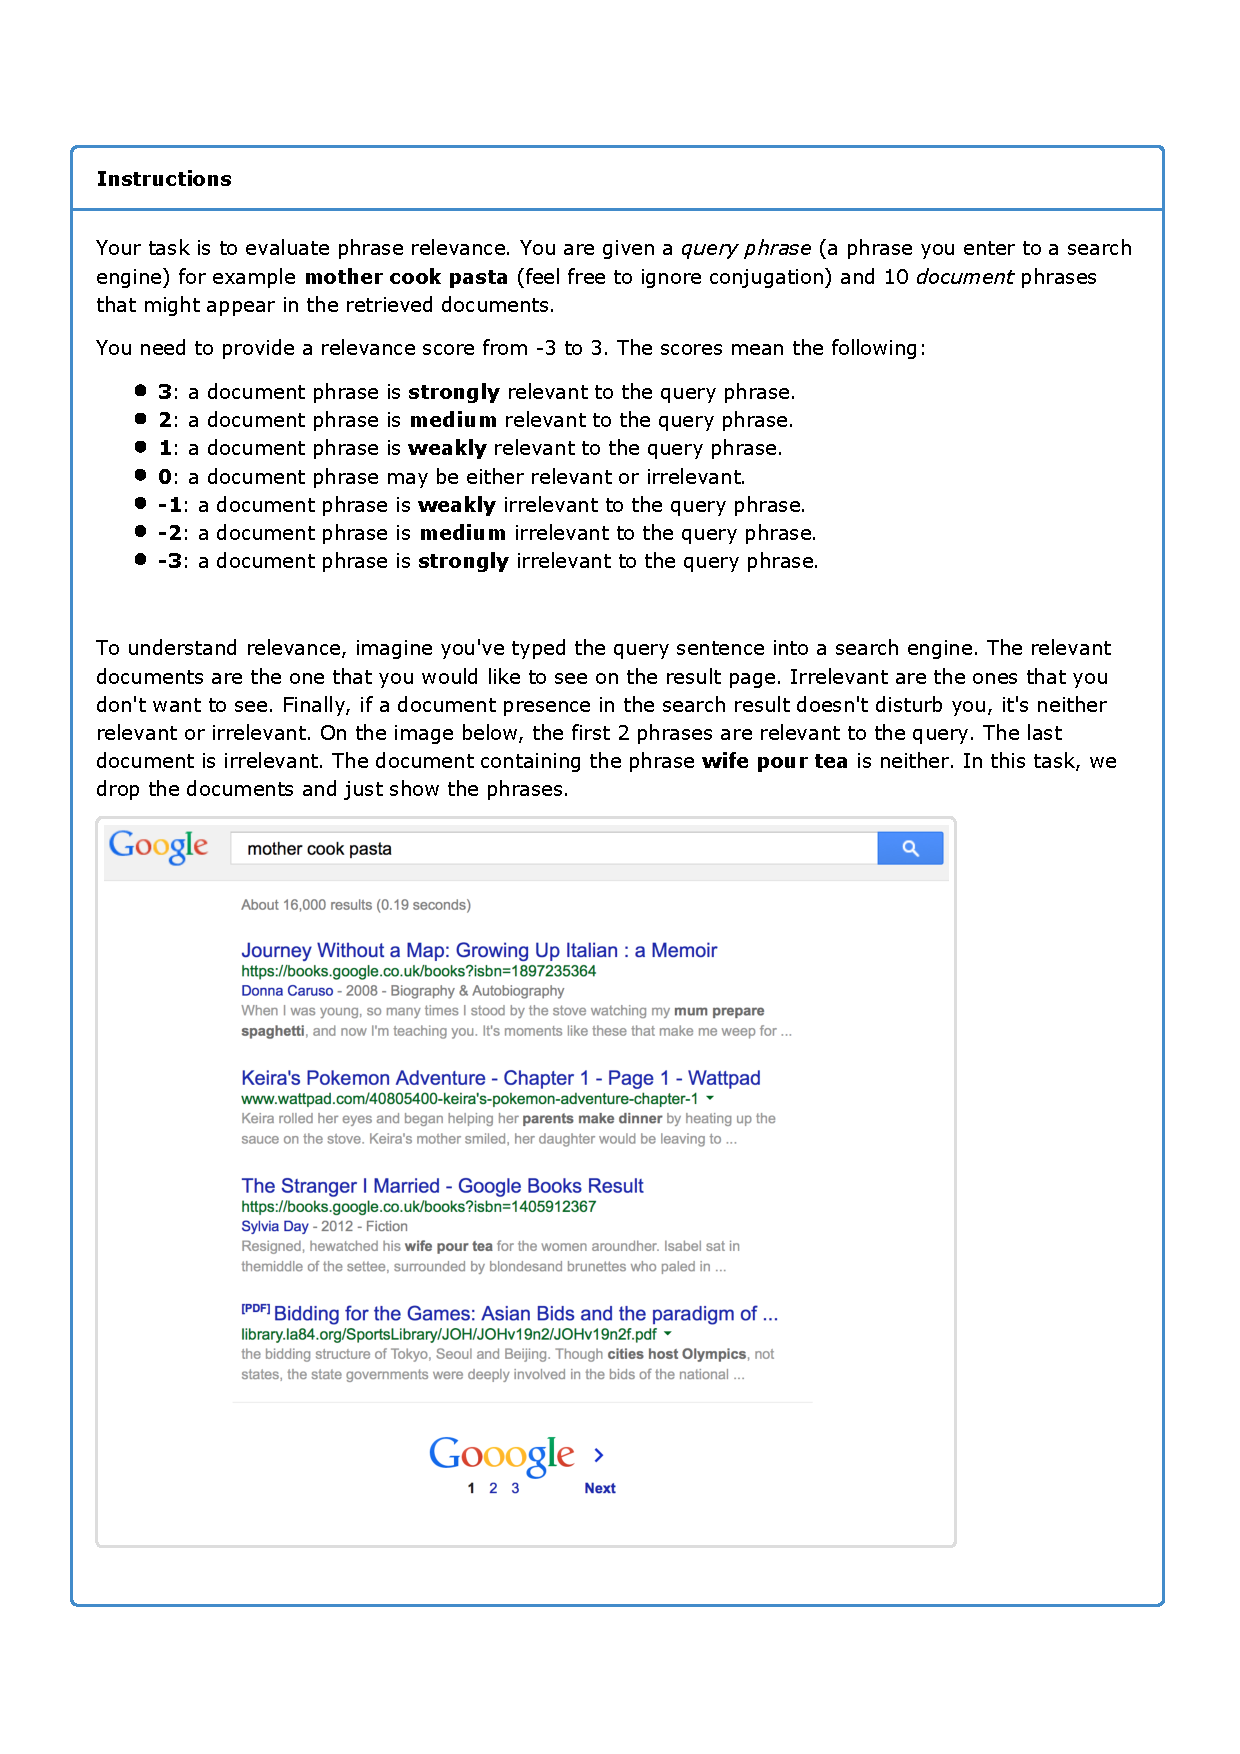
\includegraphics[width=0.9\textwidth]{figures/instructions}

\caption{Instructions given to the Mechanical Turkers}

\label{fig:instructions}
\end{figure}

%%% Local Variables:
%%% mode: latex
%%% TeX-master: "../paper.tex"
%%% End:


We recruited 19 human subjects using the Amazon Mechanical Turk platform.\footnote{\url{https://requester.mturk.com/}} Before answering a question, the subjects were given the instructions shown in Figure~\ref{fig:instructions}.

Each query-document pair was judged by three different people. The data was collected in two batches. Each question (or a HIT, Human Intelligence Task, in the Mechanical Turk terminology) consisted of a query phrase and 20 document sentences for the first batch and 10 documents for the second batch. Documents were shuffled before being shown to a human subject. Each document had to be judged for relevance using the following scoring system:
\begin{compactitem}
\item \textbf{-3}: strong irrelevance,
\item \textbf{-2}: medium irrelevance,
\item \textbf{-1}: weak irrelevance,
\item  \textbf{0}: a document may be either relevant or irrelevant,
\item  \textbf{1}: weak relevance,
\item  \textbf{2}: medium relevance,
\item  \textbf{3}: strong relevance.
\end{compactitem}

An example question is shown in Figure~\ref{fig:task}. The \dataurl{phraserel-raw.csv} file consists of human judgements together with anonymized Worker and HIT identifiers.

\begin{figure}
\centering
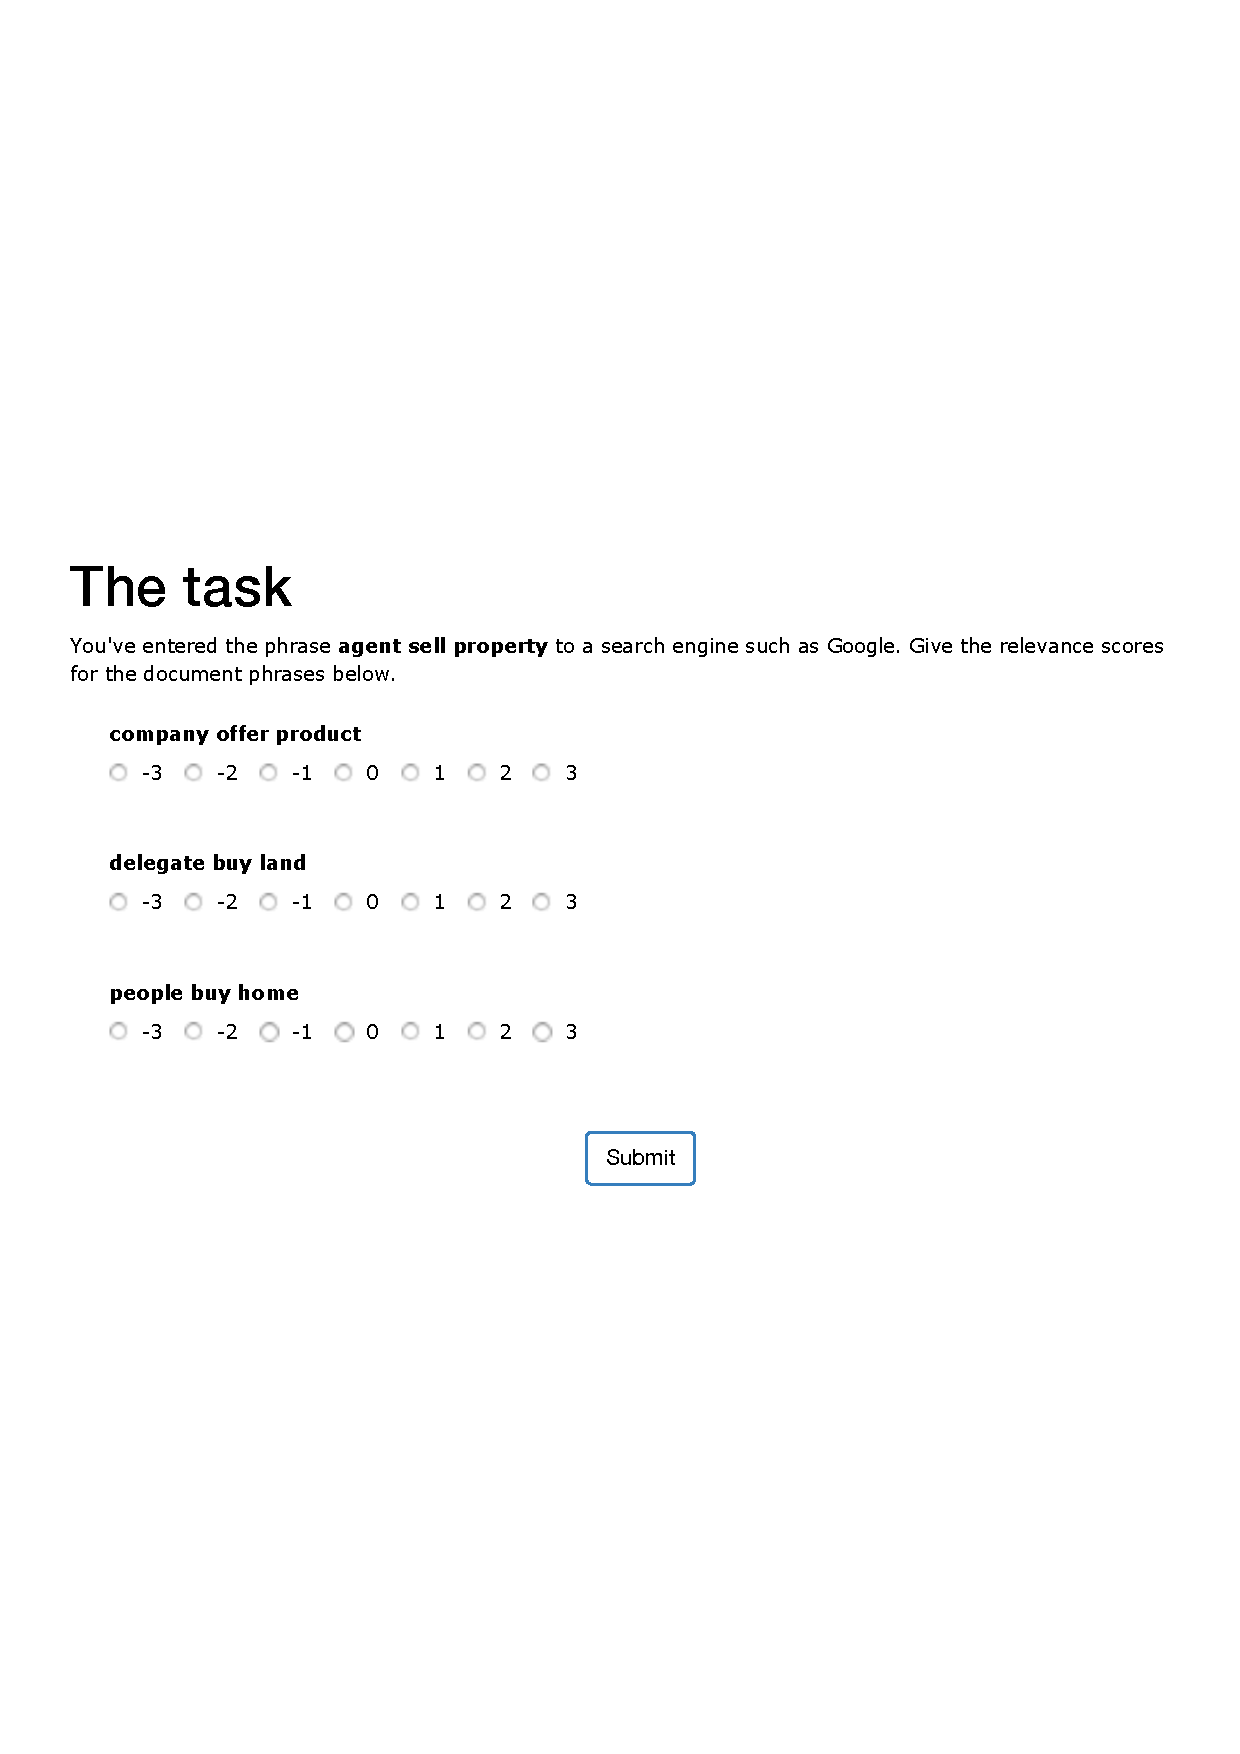
\includegraphics[width=0.9\textwidth]{figures/task}

\caption{\textbf{A sample question.}}

\label{fig:task}
\end{figure}

%%% Local Variables:
%%% mode: latex
%%% TeX-master: "../paper.tex"
%%% End:


\section{Final dataset construction}
\label{sec:postprocessing}

\subsection{Pair classification}

The pairs have been classified by the individual relevance judgements. A pair is of the \textit{strict relevance} type if all human judgements are greater than or equal to 0 and there is at least one 3 (strong relevance). A pair of the \textit{loosely   relevant} type is a pair where all human judgements are greater than or equal to 0. Figure~\ref{fig:emnlp-pairing} shows the mean and standard deviation of human judgements per query-document pair and the relevance division of a pair if applicable. There are 110 (or 7\%) strictly relevant pairs and 221 (13\%) loosely relevant pairs.
% * <sdyck@ualberta.ca> 2016-11-04T13:35:55.761Z:
%
% >  greater than or equal to 0
%
% but no 3's? otherwise loosely and strictly relevant classifications would overlap (all strictly would also be loosely) if that makes sense. 
%
% ^.

\subsection{Query classification}

Each query has been classified by the number of strictly relevant documents it has been paired with. On average, each query in the dataset is paired with 3.3 loosely relevant and 1.6 strictly relevant documents. The minimum number of loosely relevant documents per query is 1, the maximum is 14. Regarding the strict relevance, there are 8 queries without a single strictly relevant document, and the maximum number of strictly relevant documents per query is 7.

A query is \textit{diverse} if it is paired with 4 or more loosely relevant documents. There are 28 (42\%) such queries. On average, diverse queries are paired with 5.2 loosely relevant documents and 2.4 strictly relevant documents.
% \begin{compactitem}
% \item 14 queries with 4 loosely relevant documents,
% \item 6 with 5,
% \item 5 with 6,
% \item 1 with 7,
% \item 1 with 9,
% \item 1 with 14.
% \end{compactitem}

%%% Local Variables:
%%% mode: latex visual-line
%%% TeX-master: "thesis"
%%% TeX-engine: xetex
%%% End:


\cleardoublepage
\addcontentsline{toc}{chapter}{Bibliography}
\phantomsection
\bibliographystyle{plainnat}
\bibliography{references,dmilajevs_publications}

\end{document}
